Afin d'obtenir une cohérence spatiale et un environnement peu bruité, il est nécessaire d'atteindre des températures de l'ordre de quelques milliKelvins. Pour cela on utilise un cryostat à dilution sèche.
\section{Principe d'un cryostat à dilution}
\begin{figure}[h]
  \begin{center}
    \includegraphics[width=0.6\textwidth]{Images/Cryostat_Schema.pdf}
    \qquad
    \includegraphics[width=0.33\textwidth]{Images/Helium_phase_diagram.pdf}
    \caption{Schéma du cryostat à dilution et diagramme de phase du mélange d'Hélium}
  \end{center}
\end{figure}
Le cryostat à dilution est basé sur certaines propriétés du mélange des isotopes d'Hélium \HeT et \HeQ.
\newline

Prenons un mélange équilibré liquide \HeT/\HeQ(donc pré-refroidi à 1K) ; l'\HeQ étant le plus lourd, il tombe au fond et l'\HeT flotte au-dessus.

Ensuite, du point de vue des interactions quantiques dans chacun des liquides, on remarque que les interactions pour l'atome d'\HeT sont plus faibles que pour l'\HeQ : les premiers vont descendre dans la phase \HeQ, mais pas l'inverse.
\newline

On se trouve donc en présence de deux phases: celle, plus légère, d'\HeT pur, et celle de mélange \HeT/\HeQ.
Enfin, les atomes d'\HeT sont des Fermions, et le principe d'exclusion de Pauli s'y applique: la solubilité de l'\HeT dans l'\HeQ sera limitée aux environs de \{6,6\% \HeT, 93.4\% \HeQ\}.
\newline

Lorsqu'on pompe de l'\HeT de la phase diluée vers la phase pure, une pression osmotique va apparaître à l'interface des deux phases: l'\HeT va alors se dissoudre dans la phase diluée. Or cette réaction est endothermique, et ceci fournit la puissance calorifique au cryostat.

Ceci se passe au niveau de la chambre de mélange.\newline

Lorsque la pompe diminue la pression dans cette chambre de mélange, la phase diluée va monter jusqu'au réservoir supérieur. Ici, la température est aux alentours de 600-800mK et la pression de $\sim$10Pa.

L'\HeT va essentiellement s'évaporer du mélange. En effet, il a une pression partielle bien plus évelée que l'\HeQ, qui lui va en grande partie rester confiné dans le réservoir et dans la chambre de mélange.
\newline

La vapeur, constituée donc essentiellement d'\HeT, va alors passer par la pompe (à température ambiante), être refroidie pour revenir jusqu'à la chambre de mélange où la pression osmotique entre les deux phases va augmenter d'autant plus: de l'\HeT va alors passer dans la phase diluée en refroidissant le cryostat, et recommencer le processus. \newline

Les échangeurs thermiques permettent à l'\HeT réinjecté d'être remis à basse température pour ne pas réchauffer l'ensemble du cryostat. Cela permet aussi d'augmenter la température dans le réservoir supérieur et permettre à l'\HeT de s'évaporer.

Une résistance chauffante est située au niveau du réservoir, pour la même raison.

\section{Cryostat sec: Principe du tube à gaz pulsé}
Le mélange doit être pré-refroidi avant d'être injecté dans le cryostat.\newline
Il passe tout d'abord par un bain d'azote liquide à 77K qui permet aussi de nettoyer le mélange des impuretés (le "piège").

La plupart des cryostats utilisnt ensuite un bain d'\HeQ liquide à 4,2K, puis un bain d'\HeQ liquide à faible pression à 1K (diminuer la pression de l'\HeQ permet d'abaisser son point de condensation).

Ces derniers bains nécessitant un apport supplémentaire d'\HeQ, il peuvent être remplacé par un tube à gaz pulsé, d'où l'appellation de cryostat sec (mis à part le bain d'azote liquide qui est à l'extérieur du cryostat).

Un tube à gaz pulsé fonctionne selon un cycle proche du cycle de Stirling, grâce à un piston et un compresseur. Ceux-ci engendrent des vibrations importantes, qui pourraient empêcher toute mesure dans le cryostat. C'est pour cela que le tube pulsé est séparé du cryostat.

\begin{figure}[ht]
    \begin{center}
        \includegraphics[width=0.65\textwidth]{Images/Cryostat_PulseTube_Schema.png}
        \caption{Schéma du tube à gaz pulsé}
    \end{center}
\end{figure}


\begin{figure}[ht]
    \begin{center}
        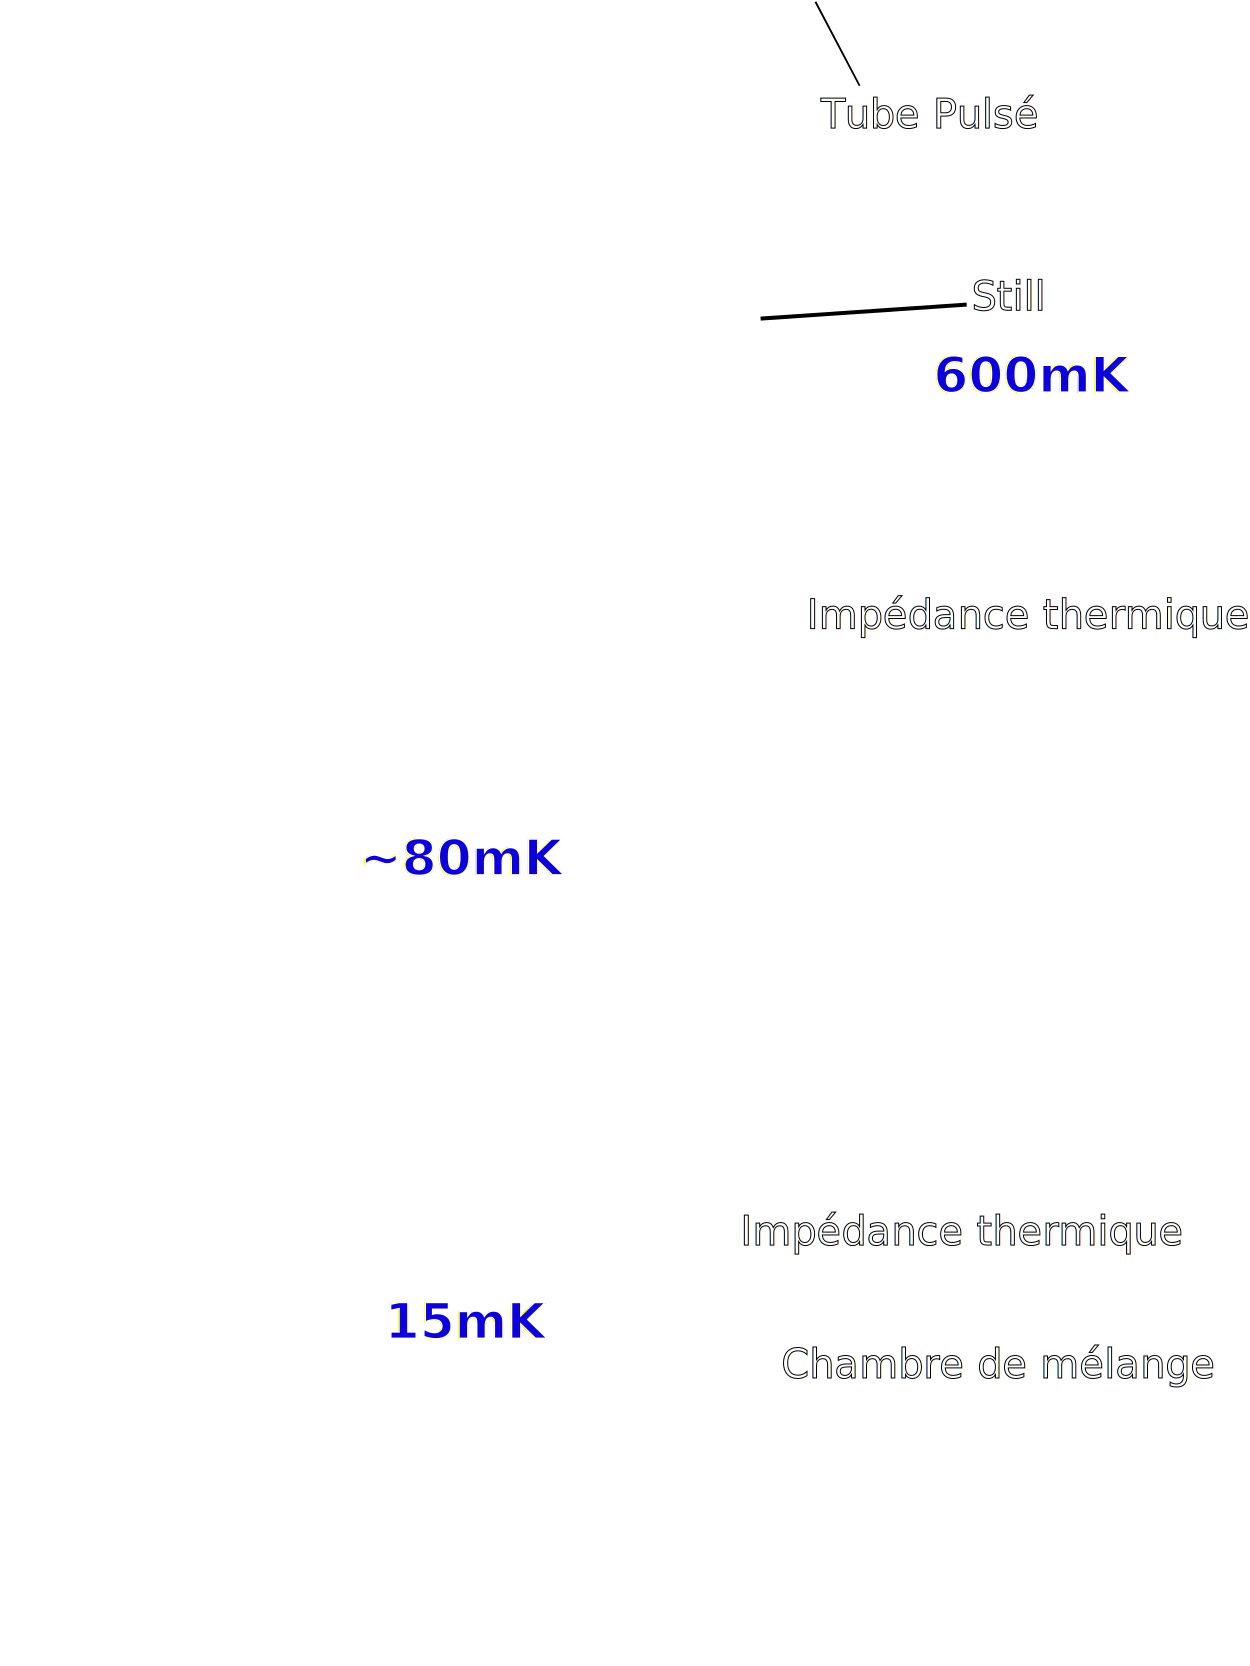
\includegraphics[width=0.75\textwidth]{Images/PhotoCryostat}
        \caption{Organisation du cryostat à dilution sèche}
    \end{center}
\end{figure}
